\section{20 Open Questions and Future Directions}\label{sec:20Q}

Current trends and future directions in smart pricing practices aim to make proposed pricing plans economically viable. For instance, substantial research has been done on day-ahead pricing, including the development of carefully designed user interfaces to display price and usage data as shown in Figure \ref{fig:tube_gui}. Incorporating human factors into the engineering and design phase along with economic models can provide a holistic approach in solving the challenges of network congestion.
%More generally, client-side architectures may ease the user burden of dynamic pricing plans; however, the design of such components remains an open problem, and this conjecture has not yet been thoroughly tested on real users.

In addition to the pricing plans proposed above, new pricing plans have recently been proposed that have been rarely studied in the academic literature. Some promising directions include the following:

\begin{figure}
\centering
\begin{subfigure}[b]{0.23\textwidth}
	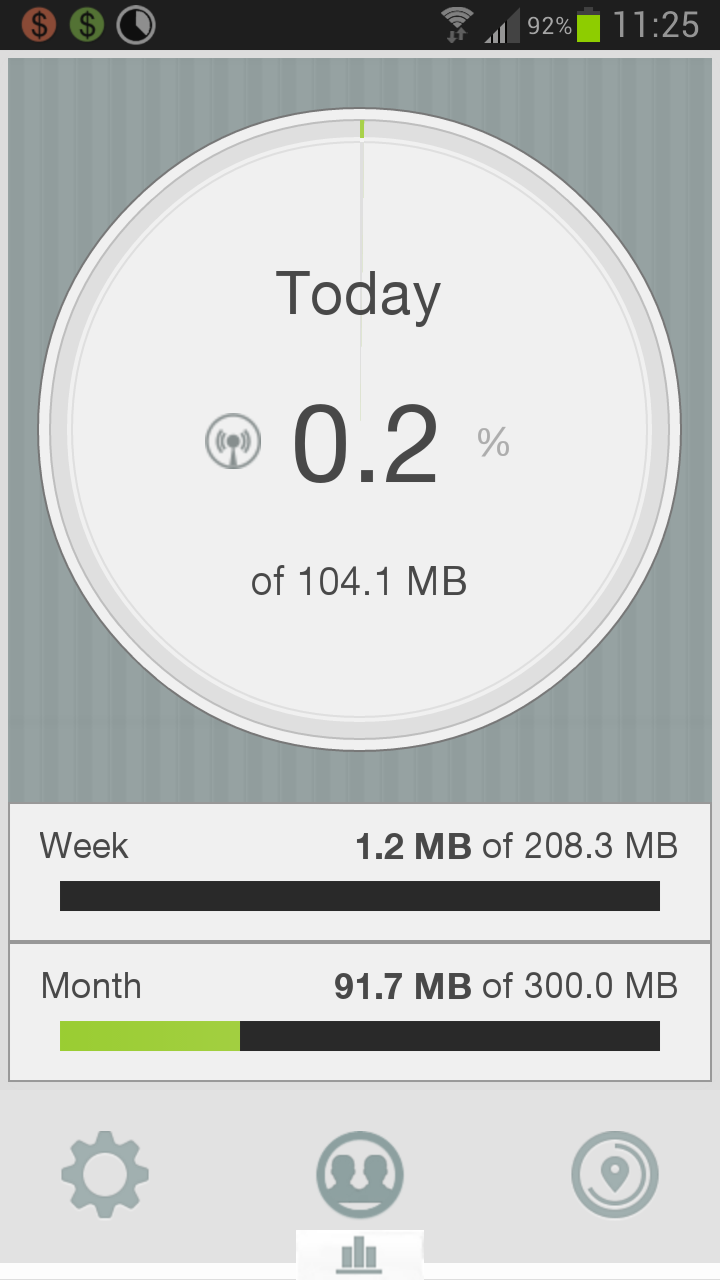
\includegraphics[width = \textwidth]{Figures/Main.png}
	\caption{Home screen.}
	%\vspace{0.05in}
	\label{fig:datawiz_main}
	\end{subfigure}
	\begin{subfigure}[b]{0.23\textwidth}
	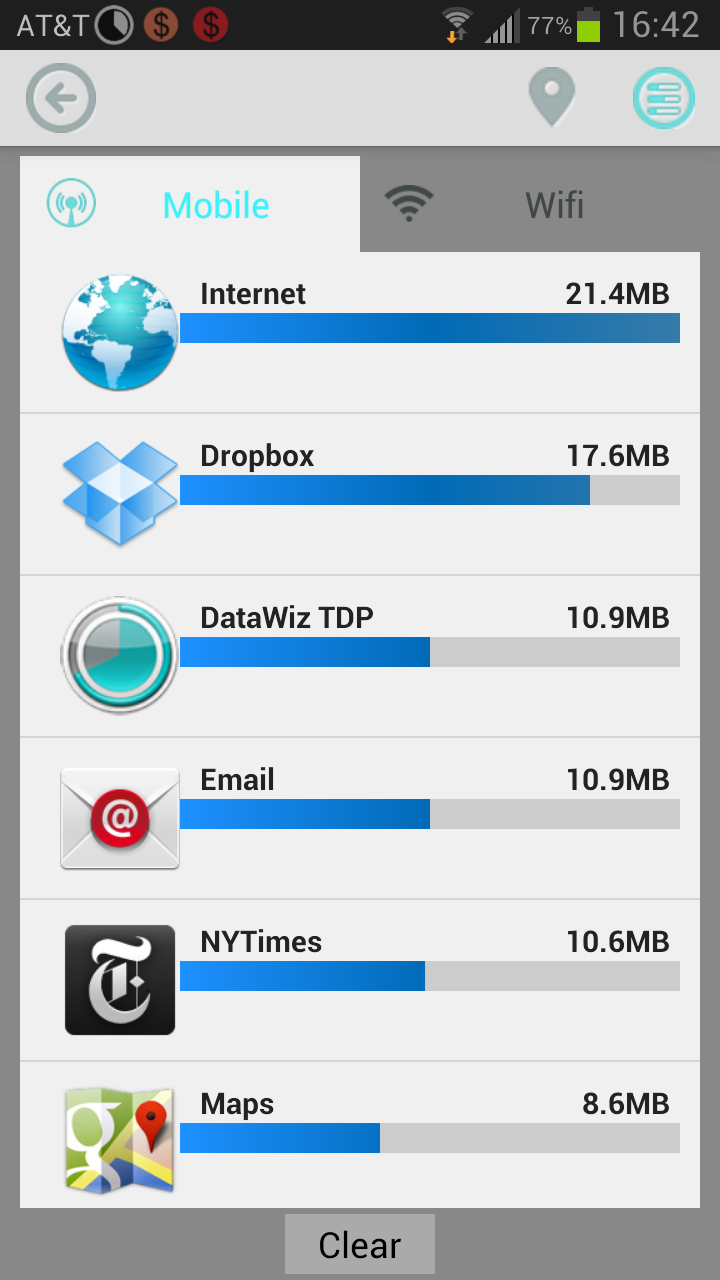
\includegraphics[width = \textwidth]{Figures/Apps_Mobile.png}
	\caption{Cellular usage per app.}
	%\vspace{0.05in}
	\label{fig:datawiz_main_graph}
	\end{subfigure}
	\begin{subfigure}[b]{0.23\textwidth}
	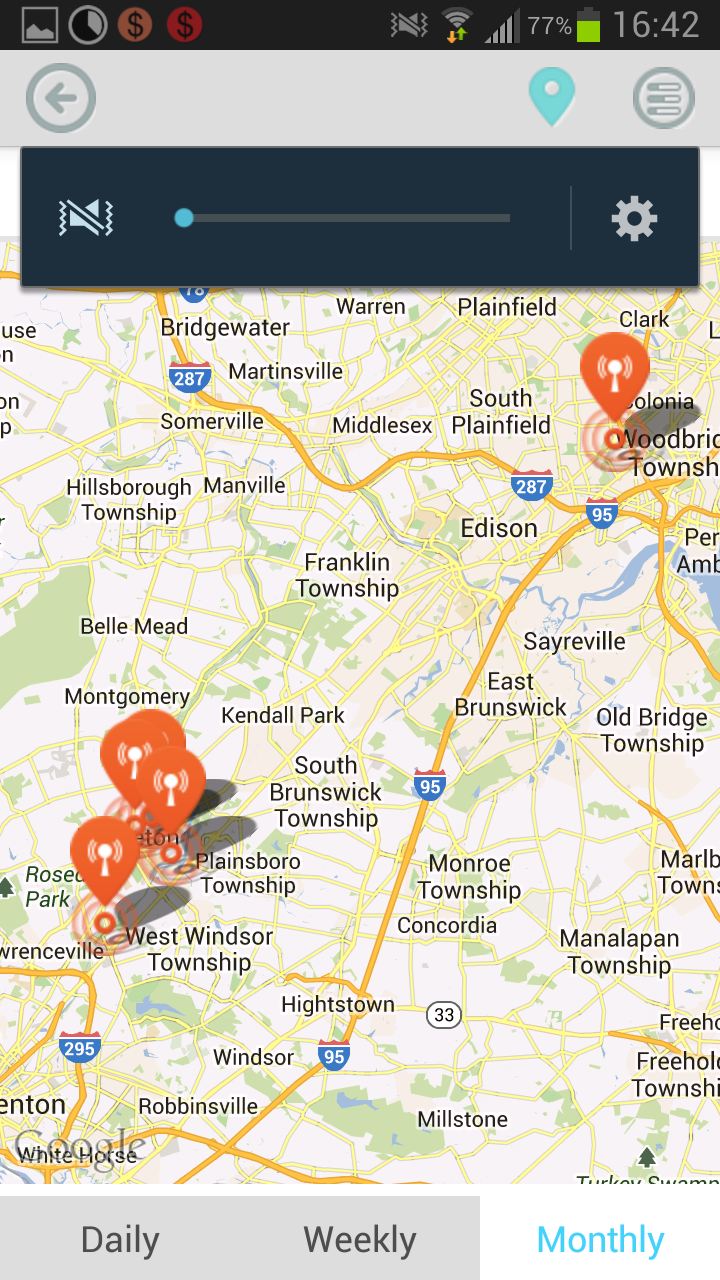
\includegraphics[width = \textwidth]{Figures/Maps.png}
	\caption{Usage locations.}
	%\vspace{0.05in}
	\label{fig:datawiz_predict}
	\end{subfigure}
	\begin{subfigure}[b]{0.23\textwidth}
	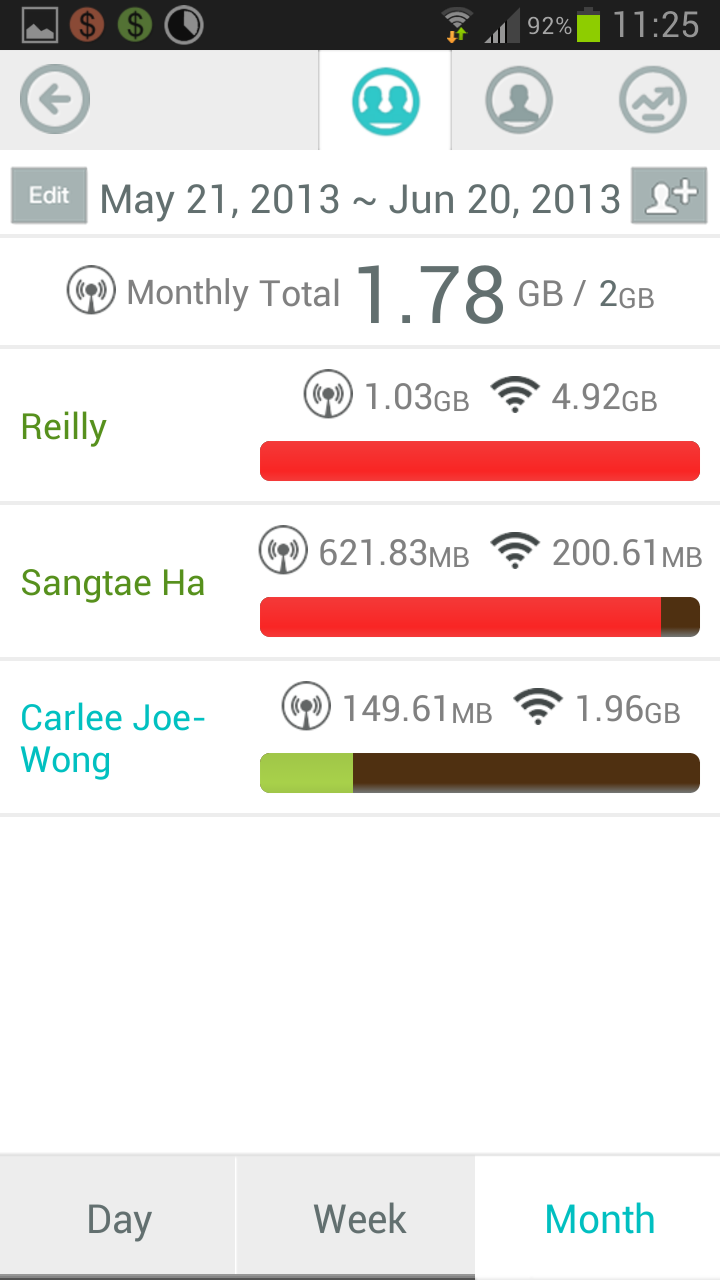
\includegraphics[width = \textwidth]{Figures/Members.png}
	\caption{Shared usage.}
	%\vspace{0.05in}
	\label{fig:datawiz_map2}
	\end{subfigure}
	
	\vspace{0.3in}
	
	\begin{subfigure}[b]{0.23\textwidth}
	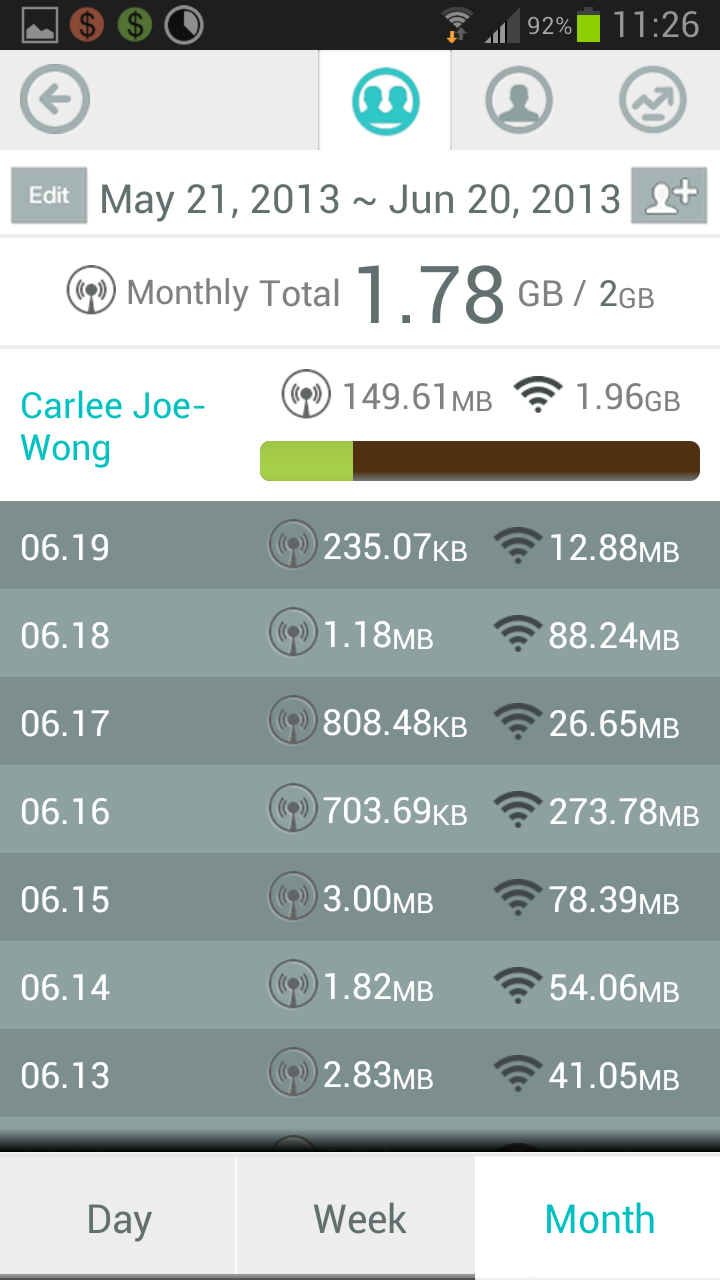
\includegraphics[width = \textwidth]{Figures/Usage.png}
	\caption{Individual usage.}
	%\vspace{-0.05in}
	\label{fig:datawiz_indv}
	\end{subfigure}
	\begin{subfigure}[b]{0.23\textwidth}
	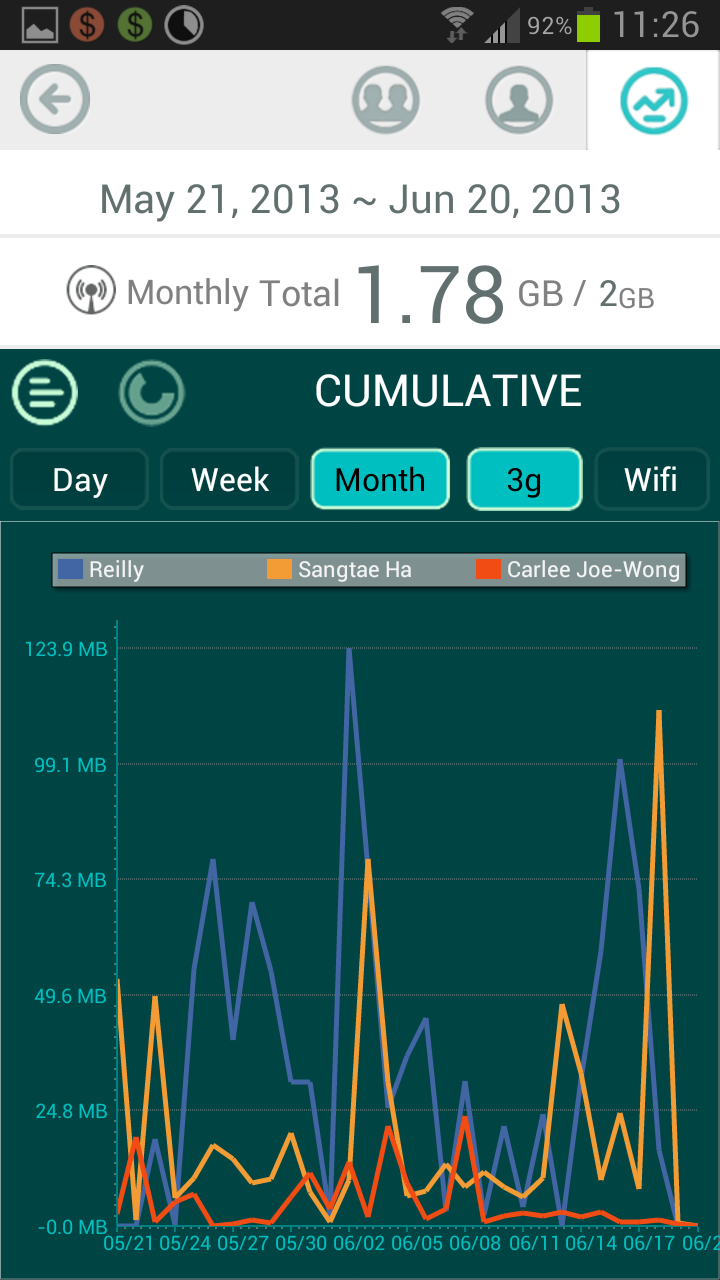
\includegraphics[width = \textwidth]{Figures/Line_Graph.png}
	\caption{Usage over time.}
	%\vspace{-0.05in}
	\label{fig:datawiz_time}
	\end{subfigure}
	\begin{subfigure}[b]{0.23\textwidth}
	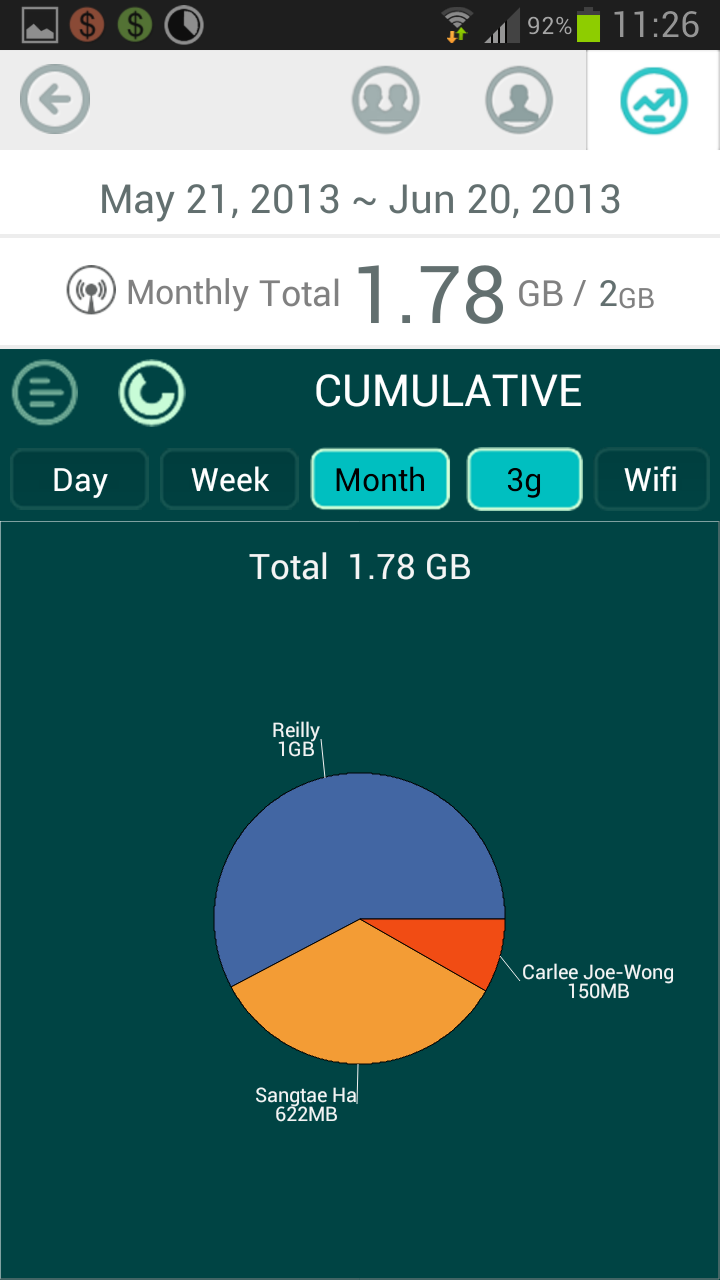
\includegraphics[width = \textwidth]{Figures/Pie_Chart.png}
	\caption{Usage distribution.}
	%\vspace{-0.05in}
	\label{fig:datawiz_pie}
	\end{subfigure}
	\begin{subfigure}[b]{0.23\textwidth}
	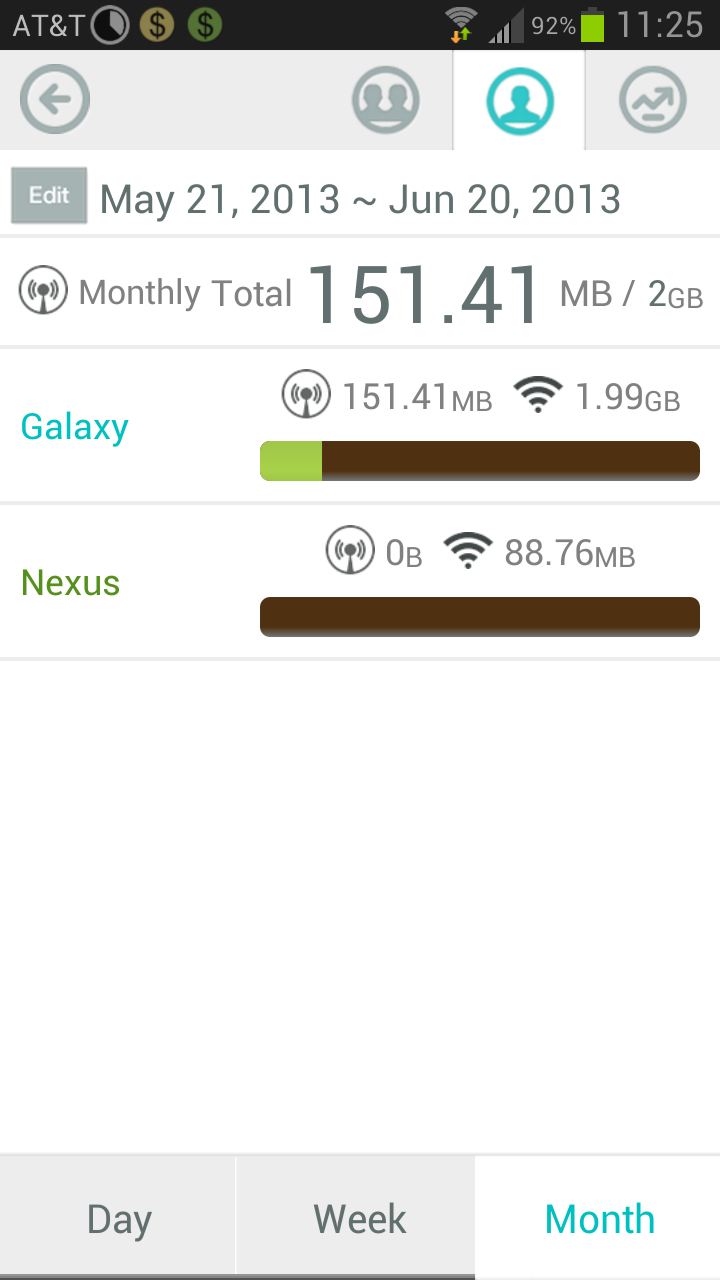
\includegraphics[width = \textwidth]{Figures/Devices.png}
	\caption{Usage of devices.}
	%\vspace{-0.05in}
	\label{fig:datawiz_device}
	\end{subfigure}
\caption{Screenshots of the DataWiz app with shared data plans. A user can add other users or devices to her shared data plan and can keep track of the shared data usage as well as individual usage. When a user is requested to be a part of the shared data plan, a push notification is sent to the user and the user can either accept or reject this invitation.}
\label{fig:datawiz}
\end{figure}

\begin{description}
\item[Shared data plans:] AT\&T and Verizon in the United States recently introduced shared data plans, in which several devices share a common data cap. While some studies of shared data plans have been made \cite{WITS}, the effects of such plans on user behavior, and how such a data cap can be shared fairly and efficiently among users, remain to be studied in detail.

One practical challenge for users on shared data plans is keeping track of their usage across multiple devices--while many apps exist to track usage on individual devices; e.g., Onavo Count, My Data Manager, and DataWiz; none track the usage of multiple devices. In fact, tracking usage on multiple devices requires not only modifications to user interface design but also integration with a common server that can send usage information of other user devices to each device on a shared plan. A login and agreement process is also necessary to ensure that users can see each others' usage only once both users have given permission.

Screenshots of a prototype shared data plan app based on the DataWiz usage monitoring application are shown in Figure \ref{fig:datawiz}. The app lets users view their monthly, weekly, and daily usage as compared to their monthly data cap (Figure \ref{fig:datawiz_main}), as well as per-app and per-location usage (Figures \ref{fig:datawiz_main_graph} and \ref{fig:datawiz_predict}). The small pie chart indicator on the top left corner of the phone allows users to quickly see their monthly usage; the chart is filled according to how much of his or her monthly cap the user has consumed.
%
In addition to these basic features, users can add and remove other users and devices to their data plan; if a user is added to someone else's data plan, the invitation recipient receives a push notification and can accept or reject the invitation. Upon acceptance, both users may view each other's usage over time (Figures \ref{fig:datawiz_indv} and \ref{fig:datawiz_time}) and on a pie chart (Figure \ref{fig:datawiz_pie}). Users may add multiple devices to their accounts; each user's total usage is then the combined usage from all of these devices (Figure \ref{fig:datawiz_device}). A push notification is sent if a user is removed from a shared data plan.

\item[Fair throttling:] Instead of merely charging users more over a certain cap, ISPs may forcibly limit usage by throttling users to a limited bandwidth rate. However, researchers have still not thoroughly examined how these bandwidth limits should be set, how they should vary over time, and what their implications are in terms of fairness across different users.

\item[Heterogeneous networks:] Many ISPs are turning to supplementary networks such as WiFi and femtocells to offload traffic from congested cellular networks. While access to such networks is often free, in the future they may wish to implement more systematic access pricing to influence the adoption of such technologies and distribution of the user population across complementary networks like WiFi and 3G \cite{wifi-3g-infocom,Im}.

\item[Sponsored content:] A major question in pricing is ``whom to charge" for delivering traffic. In a two-sided pricing model (like in the credit card business) of the Internet, the price of connectivity is shared between content providers (CPs) and end users (EUs). ISPs become the middle man (or platform) proving the connectivity between CPs and EUs. This \emph{clearing house} or data traffic exchange market would extend the existing 1-800 model of phone-call services in the USA, which charges the callee rather than the caller. The tradeoffs in the resulting economic benefit between CPs and EUs remains to be quantified. Intuitively, end-users' access prices are subsidized by third party sponsors (e.g., advertisers, content providers etc.) and the ISPs have an additional source of revenue. Perhaps more surprisingly, content providers may also stand to gain from two-sided pricing if subsidizing connectivity to end-users translates into a net revenue gain through a larger amount of consumption. However, the gain to content providers depends on the extent to which content-provider payment translates into end-users' subsidy, and on the demand elasticities of the consumers. The precise gains to the three entities will therefore depend on the respective bargaining powers stemming from their contributions and price sensitivities.

Another special case of sponsored content includes \emph{zero-rating} and \emph{1-800 reverse billing} policies for data traffic. Under zero-rating, an ISP makes certain types of application traffic available to the users for free. This kind of policy, although contentious from a net neutrality viewpoint, is a major step in app-based pricing and has been practiced in some parts of Europe (e.g., Mobistar introduced a `zero-rated' plan for Facebook, Twitter, and Netlog). Understanding the impact of such pricing plans on the network ecosystem and its neutrality are important active research directions in the area of network economics.  

% \item[Time-dependent pricing:] Day-ahead pricing for mobile data has been found to be both acceptable to users and effective at reducing the network's peak load in a small pilot trial \cite{ha2012tube}. Yet it remains to be seen whether these results hold for a larger sample of users.
\end{description}

\subsection{Static Pricing}

Usage-based static pricing has traditionally been offered by ISPs around the world, and is in some sense the simplest and least controversial form of SDP. Yet even simple caps on monthly usage require a means to communicate those caps to users and, on the ISP side, accounting infrastructure to keep track of users' remaining quotas. Pricing plans like token bucket pricing or negotiated contracts require even more interaction with end users, leading to questions that include:
\begin{enumerate}
\item
How can users use their quota efficiently and keep track of a monthly usage quota?
\item
If users choose different QoS levels or times to receive better QoS, e.g., in Paris metro or token bucket pricing, how can they do so without much technical knowledge of what ``QoS''  means? How can the ISP's infrastructure keep track of users' choices and offer the appropriate QoS?
\item
Without such technical knowledge, how can users negotiate contracts (e.g., cumulus pricing) with ISPs? How can ISPs enforce these contracts?
\item
If the ISP offered some form of personalized (e.g., app-based) pricing, how would it measure the usage of different applications for each user? Where in the network should such measurements take place (i.e., client devices or the network core)? From a regulatory perspective, does this violate privacy or network neutrality concerns?
\item
How will users share the monthly data quotas imposed by shared data plans among different devices?
\end{enumerate}
%Many ISPs and third party developers, including a team led by the authors, have already released mobile apps that tell users how much of their monthly quota is left \cite{datawiz}. Yet the effects of such applications are still unclear, and little research has been done on the \emph{design} of such apps. Similarly, there has been relatively little work on automating QoS choices or negotiations for users, and the feasibility of app-based pricing or other personalized data plans remains in question.

\subsection{Dynamic Pricing}
While static pricing offers some challenges in communicating between ISPs and end users, dynamic pricing introduces even more complications as the user must be informed of changes in price. Deployment questions unique to dynamic pricing include:
\begin{enumerate}
\setcounter{enumi}{5}
\item
How often should the prices change? Should they change with the network congestion, or should they change only after a fixed time interval (e.g., one hour)?
\item
Should users be told the prices in advance? Will they accept or respond to prices that change in real time?
\item
The answer to the previous question can be more broadly phrased as follows--how can users be appropriately informed of the changing prices (e.g., with an app on their mobile devices)? What kind of design is optimal for such an app? Going further, what mechanisms can be developed to help users adjust their behavior in response to the prices?
\item
In the context of mobile data, network bottlenecks are generally highly location-dependent. Should the prices vary by location as well as by time? How will this affect users who move from one location to another?
\item
How can the prices be computed efficiently? Should this computation be done online or offline? What usage monitoring must take place, and how real time does it need to be?
\item
In addition to efficient usage monitoring, how can the ISP anticipate user reactions to the prices so as to set the ``optimal" prices? How can these change over time? Does the measurement process adequately protect user privacy?
\item
Should dynamic pricing be coupled to QoS? If so, how?
\end{enumerate}
%A recent trial of day-ahead time-dependent pricing for mobile data addressed some of these questions by implementing hourly changes in prices, which are fixed one day in advance \cite{ha2012tube}. The prices were calculated based on aggregated usage and observed changes in aggregate usage for different pries offered, so as to make the computation scalable and protect individual users' privacy. The trial included the implementation of a client-side app that showed users their price and usage history and automatically scheduled some applications to cheaper times of the day so as to keep users' monthly expenses below a maximum budget. Yet this trial involved relatively few participants, and it did not address such questions as location-dependent bottlenecks or QoS coupling.

\subsection{Sponsored Content}

% While they look quite different in practice, both sponsored content and fair throttling naturally accommodate with content providers and government regulators, perhaps more than other forms of SDP. Thus, several unique questions arise for these particular pricing plans:
Sponsored content pricing, in which content providers and advertisers subsidize users' spending on data, has not been widely deployed, partially due to the network neutrality implications of content provider subsidies. As a relatively new type of pricing, many questions remain to be answered:
\begin{enumerate}
\setcounter{enumi}{12}
\item
What is the preferred mode of ``sponsoring'' in sponsored content/access? Should it be based on increasing the user's data cap, monetary discounts, or improved speed (e.g., less throttling)?
\item
Will content providers sponsor content on a per-transaction basis? If so, how should these transactions be metered, and how much should they charge?
\item
How can ISPs measure the cost of each transaction and develop accounting systems to keep track of content providers' sponsorship?
\item
Does the idea of ``sponsored content'' violate network neutrality? Or can it be structured in a net-neutral way, e.g., sponsoring some data usage but not specifying the application?
\end{enumerate}

\subsection{Fair Throttling and Heterogeneous Networks}

Other solutions to network congestion that do not explicitly use SDP include fair throttling and deployment of heterogeneous networks to offload traffic. Fair throttling has not been widely deployed in practice--while many ISPs do throttle users who exceed a certain usage cap, such measures are fairly crude and do not take into account users' full profiles. More sophisticated throttling, e.g., Comcast's throttling of Netflix traffic in 2007, has been controversial. In contrast, many ISPs have begun offering WiFi hotspots, but it remains unclear how effective they are in relieving congestion on mobile networks. Thus, interesting theoretical and implementation questions remain for both these types of pricing, including the following:
\begin{enumerate}
\setcounter{enumi}{16}
\item
What criteria should the ISP consider when performing ``fair'' throttling? Does measuring these criteria violate user privacy or network neutrality (e.g., throttling based on the usage of specific application types)?
\item
Should users be directly involved in prioritizing different types of traffic? How can their preferences be incorporated into the throttling algorithm without the act of declaring such preferences becoming onerous to the user?
\item
How much traffic can be offloaded to other heterogeneous networks (e.g., 4G traffic to WiFi)? How cost effective is deploying such networks as a solution to network congestion? How can ISPs estimate the monetary and spectral benefits achieved through such traffic offloading or demand shifting?
\item
If ISPs were to charge for bundled access to supplementary networks like WiFi hotspots, how would such pricing plans affect users' adoption and the overall network congestion?
\end{enumerate}

These 20 questions are only some of the key questions that arise in deploying SDP and can help researchers identify interesting topics for exploration. In the coming years, as the Internet evolves further, answering these questions and others that emerge will help determine how we access (and pay for) the Internet in a highly connected, data-driven world. 
